\chapter{Market Understanding and Data Selection}

This chapter, I will briefly illustrate the characteristics of Hong Kong stock market. After that, some introduction about the parameters I choose for this dissertation

\section{Introduction of Hong Kong Stock Exchange market}

\begin{figure}[h]
	\centering
	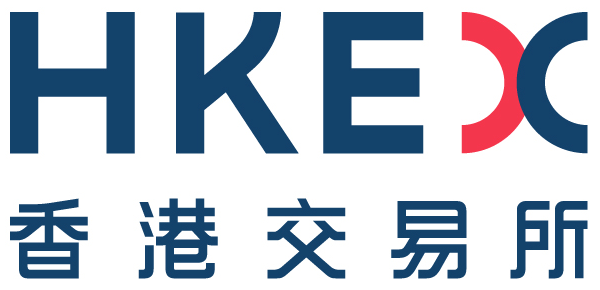
\includegraphics[width=0.5\textwidth]{hkexlogo}
	\caption{logo of HKEX}
\end{figure}

Hong Kong Exchanges and clearing Limited, or HKEX, is a stock exchange operator and clearing houses located in Hong Kong. Its ability of securities can be traced back to the foundation of the Association of Stockbrokers in Hong Kong in 1891\cite{1_history_hkex_markets_2016}.\\

HKEX is now one of the largest operators all over the world. By the end of 2015, there are 1866 companies listed on HSI, 951 of which are from mainland China, and HKEX’s total market capitalization is around HK\$24.68trillion\cite{hkex_fact_book_2015}.\\

As a developed market, the efficiency of HKEX has already been proved \cite{su2015efficiency}. This give our study a great convenient.
